\documentclass[11pt, a4paper]{MATH2023}
\usepackage{fancyhdr}
\usepackage{setspace}
\usepackage{amsmath,mathrsfs}
\usepackage{multicol}
\usepackage{amssymb}
\usepackage{graphicx}
\usepackage{caption}
\usepackage{subcaption}
\usepackage{xcolor}
\usepackage{enumitem}
\usepackage{tikz}
\usepackage{mathtools}
\usetikzlibrary{matrix}
\usepackage[normalem]{ulem}
\usepackage{multirow}
\usepackage{esint}      % \varoiint
\usepackage[linesnumbered, ruled, boxed]{algorithm2e}
\SetKwRepeat{Do}{do}{while}
\newcommand{\eg}{\textbf{[Example.] }}
\newcommand{\sol}{\textbf{[Solution.] }}
\newcommand{\ii}{{\bf i}}
\newcommand{\jj}{{\bf j}}
\newcommand{\kk}{{\bf k}}
\newcommand{\rr}{{\bf r}}
\newcommand{\FF}{{\bf F}}
\newcommand{\nm}{\widehat{\bf n}}
\renewcommand{\div}{{\rm div\ }}
\newcommand{\curl}{{\rm curl\ }}
\newcommand{\pt}{\partial}


\title{Chapter 16}
\subtitle{Vector Calculus}

\begin{document}
\begin{spacing}{1.3}

    \section{The Divergence Theorem}

    Let $G$ be a simple solid whose boundary surface $S$ has {\it positive (outward)} orientation.
    When we find the {\bf flux} of $S$ in a {\it smooth} vector field
    $\FF(x,y,z)=f(x,y,z)\ii + g(x,y,z)\jj +h(x,y,z)\kk$, 
    the {\bf Divergence Theorem} gives:
    \begin{center}
        \boxed{$$\disp \varoiint_S  \FF\cdot \nm\ dS=\iiint_G \nabla\cdot \FF\ dV$$}
    \end{center}
    where $\nm$ is a unit normal vector pointing out of $G$.

    In other words, {\it the total divergence within $G$ equals the net flux emerging from $G$.}

    \vspace{0.5in}
    Moreover, if the volume is very small, we can assume $\nabla\cdot \FF$ is {\it constant} within 
    the small volume, thus 
    \begin{align*}
        \varoiint_{\delta S}\FF\cdot \nm \ dS &= \nabla \cdot \FF \iiint_{G}\ dV \\
        &= \nabla\cdot \FF \cdot \delta V
    \end{align*}
    Therefore, $$\nabla\cdot \FF =\lim_{\delta V\rightarrow 0} \frac{1}{\delta V}
    \varoiint_{\delta S} \FF\cdot \nm \ dS$$

    This is the definition of divergence given in lecture note Chapter 15.

    \vspace{0.7in}
    {\it Since exam will not cover the proof, I'd like to omit here.}


    \newpage
    {\blue This example shows how Divergence Theorem simplifies the computation of flux.}



    \newpage
    \section{Green's Theorem}
    \subsection{Green's Theorem in Line Integral}

    {\blue In this part, we will go back to {\bf line integral}, which we have done a lot.}

    Now consider doing line integral in a smooth simple {\bf closed curve} $C$ in the $xy$-plane,
    if $\FF(\rr)=P(\rr)\ii+Q(\rr)\jj$, then if we want to evaluate $\disp \oint_C\FF\cdot d\rr$,
    \begin{center}
        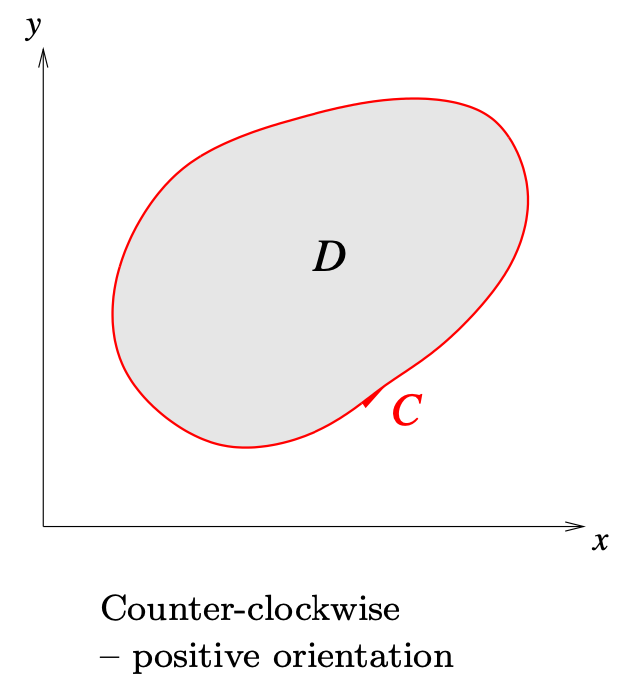
\includegraphics[scale=0.43]{images/Ch16-green-closed-path.png}
    \end{center}
    \begin{itemize}
        \item If $\FF$ is conservative, then line integral is 0, obviously.
        \item If $\FF$ is not conservative, then {\bf Green's Theorem} tells us 
        \begin{center}
            \boxed{$$\disp \oint_C \FF\cdot d\rr=\iint_D (\nabla \times \FF)\cdot \kk\ dA$$}
        \end{center}
    \end{itemize}
    {\bf Note} $\kk$ is the {\bf normal} to $xy$-plane, or, normal to region $D$.

    \vspace{0.3in}
    {\it Since exam will not cover the proof, I'd like to omit here.}

    
    
    
    \newpage
    {\blue This example shows how Green's Theorem simplify computation.}

    \eg $\disp \int_{C} x y d x+2 x^{2} d y$, $C$ consists of the segment from $(-2,0)$ to $(2,0)$ and top half of the circle
    $x^2+y^2=4$.
    \begin{center}
        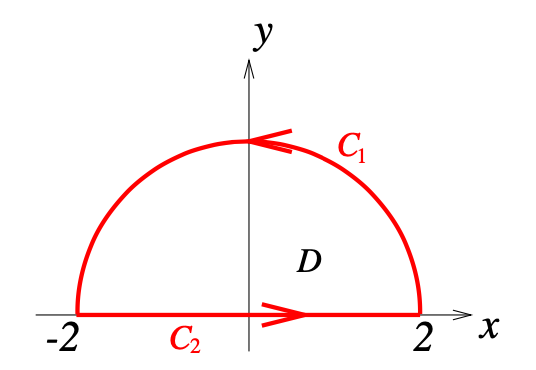
\includegraphics[scale=0.45]{images/Ch16-ex4.2.png}
    \end{center}
    
    \sol 
    
    {\bf Method 1:} use line integral: 
    $$ \int_{C} x y d x+2 x^{2} d y=\int_{C_{1}} x y d x+2 x^{2} d y+\int_{C_{2}} x y d x+2 x^{2} d y$$
    Parametrize the two curves:
    \begin{align*}
        C_{1} &: \mathbf{r}(t)=(1-t)(-2,0)+t(2,0)=(4 t-2,0) \quad 0 \leqslant t \leqslant 1 \\
        C_{2} &: \mathbf{r}(t)=(2 \cos t, 2 \sin t) \quad 0 \leqslant t \leqslant \pi
    \end{align*}
    Then directly evaluate the two line integrals
    \begin{align*}
        \int_{C_{1}} x y d x+2 x^{2} d y &=\int_{0}^{1}(4 t-2) \cdot 0 \cdot 4 d t+2(4 t-2)^{2} \cdot(0)=0 \\
        \int_{C_{2}} x y d x+2 x^{2} d y &=\int_{0}^{\pi}(2 \cos t)(2 \sin t)(-2 \sin t) d t+2(2 \cos t)^{2}(2 \cos t) d t \\
        &=8 \int_{0}^{\pi}\left(-\cos t \sin ^{2} t+\cos ^{3} t\right) d t=0
    \end{align*}
    Thus $\disp \int_{C} x y d x+2 x^{2} d y=0$.
    
    \vspace{0.5in}
    {\bf Method 2: } using Green's theorem:

    $\FF=(xy, 2x^2)$, hence $\nabla \times \FF=(4x-x)\kk =3x\kk$, then
    \begin{align*}
        \oint_{C} x y d x+2 x^{2} d y = \iint_D 3x dA &=\int_0^2\int_0^{\pi} 3r\cos\theta \ rd\theta dr \\
            &= \left. \int_0^2 3r^2\sin\theta \right|_0^{\pi} dr=0
    \end{align*}
    Actually, one may observe that $\disp \iint_D 3x dA=0$ directly, since $3x$ is a {\it odd} function in 
    $x$, and the region $D$ is {\it symmetric with respect to }$y$-axis.



    \newpage
    \subsection{Green's Theorem for computing Area}

    Recall that Green's Theorem states that:
    $$\oint_C \FF\cdot d\rr=\iint_D (\nabla \times \FF)\cdot \kk\ dA$$
    Notice if $\FF(\rr)=P(\rr)\ii+Q(\rr)\jj$,
    $$\oint_{C} \mathbf{F} \cdot d \mathbf{r}=\oint_{C} P d x+Q d y
    =\iint_{D}\left(\frac{\partial Q}{\partial x}-\frac{\partial P}{\partial y}\right) d A
    =\iint_D (\nabla \times \FF)\cdot \kk\ dA$$

    When $\disp \frac{\pt Q}{\pt x}-\frac{\pt P}{\pt y}=1$, then 
    \begin{center}
        \boxed{$$\disp A=\iint_D dA=\oint_C Pdx+Qdy$$.}
    \end{center}

    For example, when $P=0, Q=x$, or when $P=-y, Q=0$, or when $P=-y/2, Q=x/2$,
    $$A=\oint_C xdy=-\oint_C ydx=\frac{1}{2}\oint_C xdy-ydx$$



    \newpage
    {\blue The two examples below shows how to use Green's Theorem to find area.}

    \eg Find the area of $\disp \frac{x^2}{a^2}+\frac{y^2}{b^2}=1.$

    \sol Firstly parametrize the curve, let $x=a\cos\theta,\ y=b\sin\theta,\ 0\le \theta\le 2\pi$, then 
    $$C:\ \rr(\theta)=(a\cos\theta, b\sin\theta),\ 0\le \theta\le 2\pi$$,
    If we choose $\disp \FF(\rr)=P(\rr)\ii+Q(\rr)\jj=-\frac{y}{2}\ii+\frac{x}{2}\jj$, then we have
    $$\frac{\pt Q}{\pt x}-\frac{\pt P}{\pt y}=\frac{1}{2}+\frac{1}{2}=1$$
    Hence, 
    \begin{align*}
        D &= \frac{1}{2} \oint (xdy-ydx)\\
        &= \frac{1}{2} \left[ \int_0^{2\pi} a\cos\theta\cdot b\cos\theta\ d\theta 
        + b\sin\theta\cdot a\sin\theta\ d\theta \right]\\
        &= \frac{1}{2} ab \cdot \int_0^{2\pi} (\cos^2\theta+\sin^2\theta)\ d\theta =\pi ab
    \end{align*}


    \vspace{\fill}
    \eg Find the area of the hypocycloid $x^{2 / 3}+y^{2 / 3}=a^{2 / 3}$.
    \begin{center}
        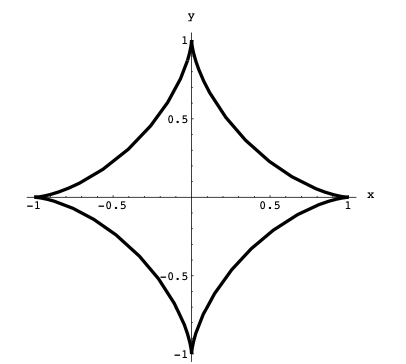
\includegraphics[scale=0.55]{images/Ch16-green-area-eg2.png}
    \end{center}

    \sol 
    Firstly parametrize the curve, 
    let $x=a \cos ^{3} \theta, y=a \sin ^{3} \theta, \quad$ where $0 \leqslant \theta \leqslant 2 \pi$,

    Again, use vector field $\disp \FF(\rr)=P(\rr)\ii+Q(\rr)\jj=-\frac{y}{2}\ii+\frac{x}{2}\jj$,
    \begin{align*}
        A=\frac{1}{2} \oint_{C} x d y-y d x &=\frac{1}{2} \int_{0}^{2 \pi}\left(a \cos ^{3} \theta \times 3 a \sin ^{2} \theta \cos \theta d \theta+a \sin ^{3} \theta \times 3 a \cos ^{2} \theta \sin \theta d \theta\right) \\
        &=\frac{3}{2} a^{2} \int_{0}^{2 \pi}\left(\cos ^{4} \sin ^{2} \theta+\sin ^{4} \theta \cos ^{2} \theta\right) d \theta \\
        &=\frac{3}{2} a^{2} \int_{0}^{2 \pi} \frac{1}{4} \sin ^{2} 2 \theta d \theta \\
        &=\frac{3}{8} a^{2} \int_{0}^{2 \pi}\left(\frac{1-\cos 4 \theta}{2}\right) d \theta=\frac{3 \pi}{8} a^{2}
    \end{align*}



    \newpage
    \subsection{General version of Green’s Theorem}

    {\blue {\it This part will not be covered in exam.}}

    Recall that Green's Theorem only applies to {\it simple} and {\it closed} curve. 
    However, it can be extended to apply to region with holes. We simply cut the region 
    into some regions that without holes, for example:
    \begin{center}
        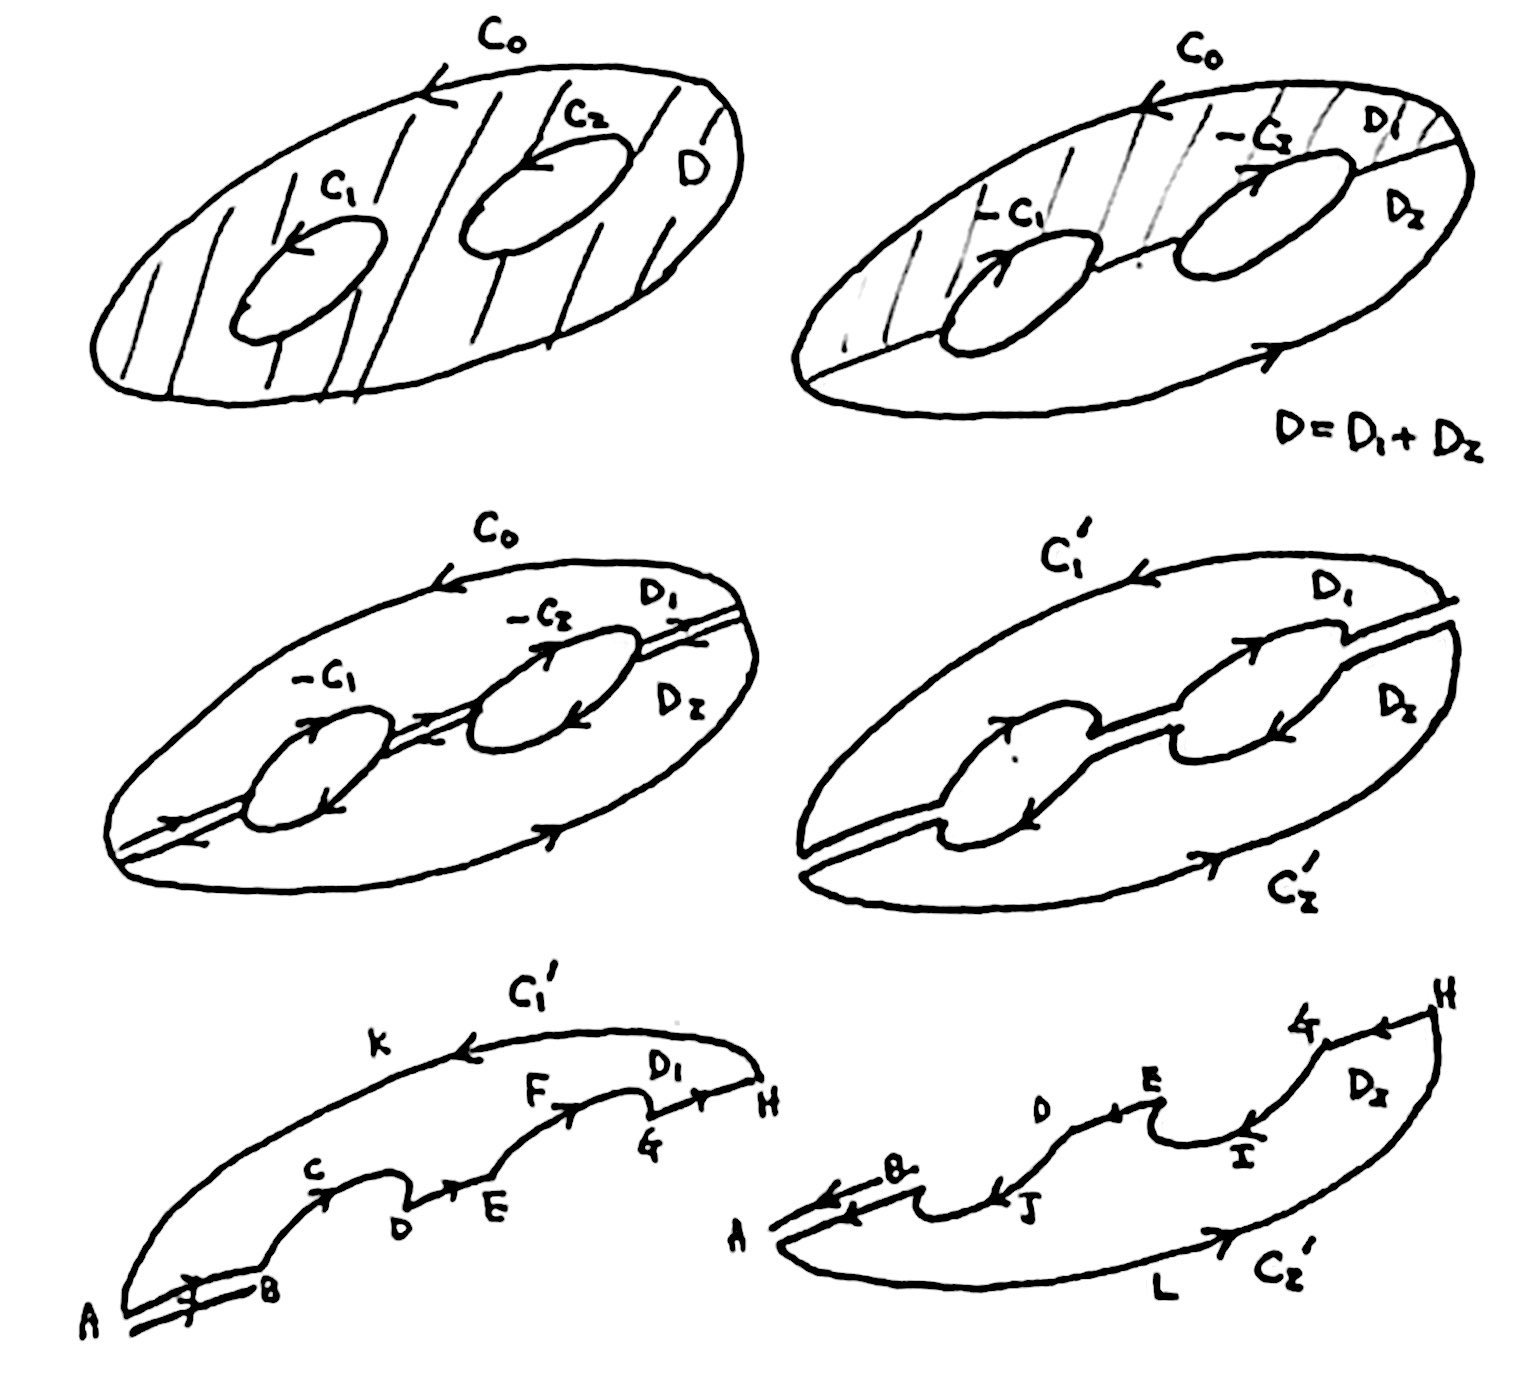
\includegraphics[scale=0.23]{images/Ch16-general-green.JPG}
    \end{center}
    \begin{align*}
        \iint_D &= \iint_{D_1}+\iint_{D_2} = \oint_{C_1^\prime}+\oint_{C_2^\prime}\\
        &= \left( \int_{HKA}+\int_{AB}+\int_{BCD}+\int_{DE}+\int_{EFG}+\int_{GH} \right)
        + \left( \int_{ALH}+\int_{HG}+\int_{GIE}+\int_{ED}+\int_{DJB}+\int_{BA} \right)\\
        &= \int_{C_0}-\int_{C_1}-\int_{C_2}
    \end{align*}



    \newpage
    {\blue Here is the example provided in lecture note.}
    
    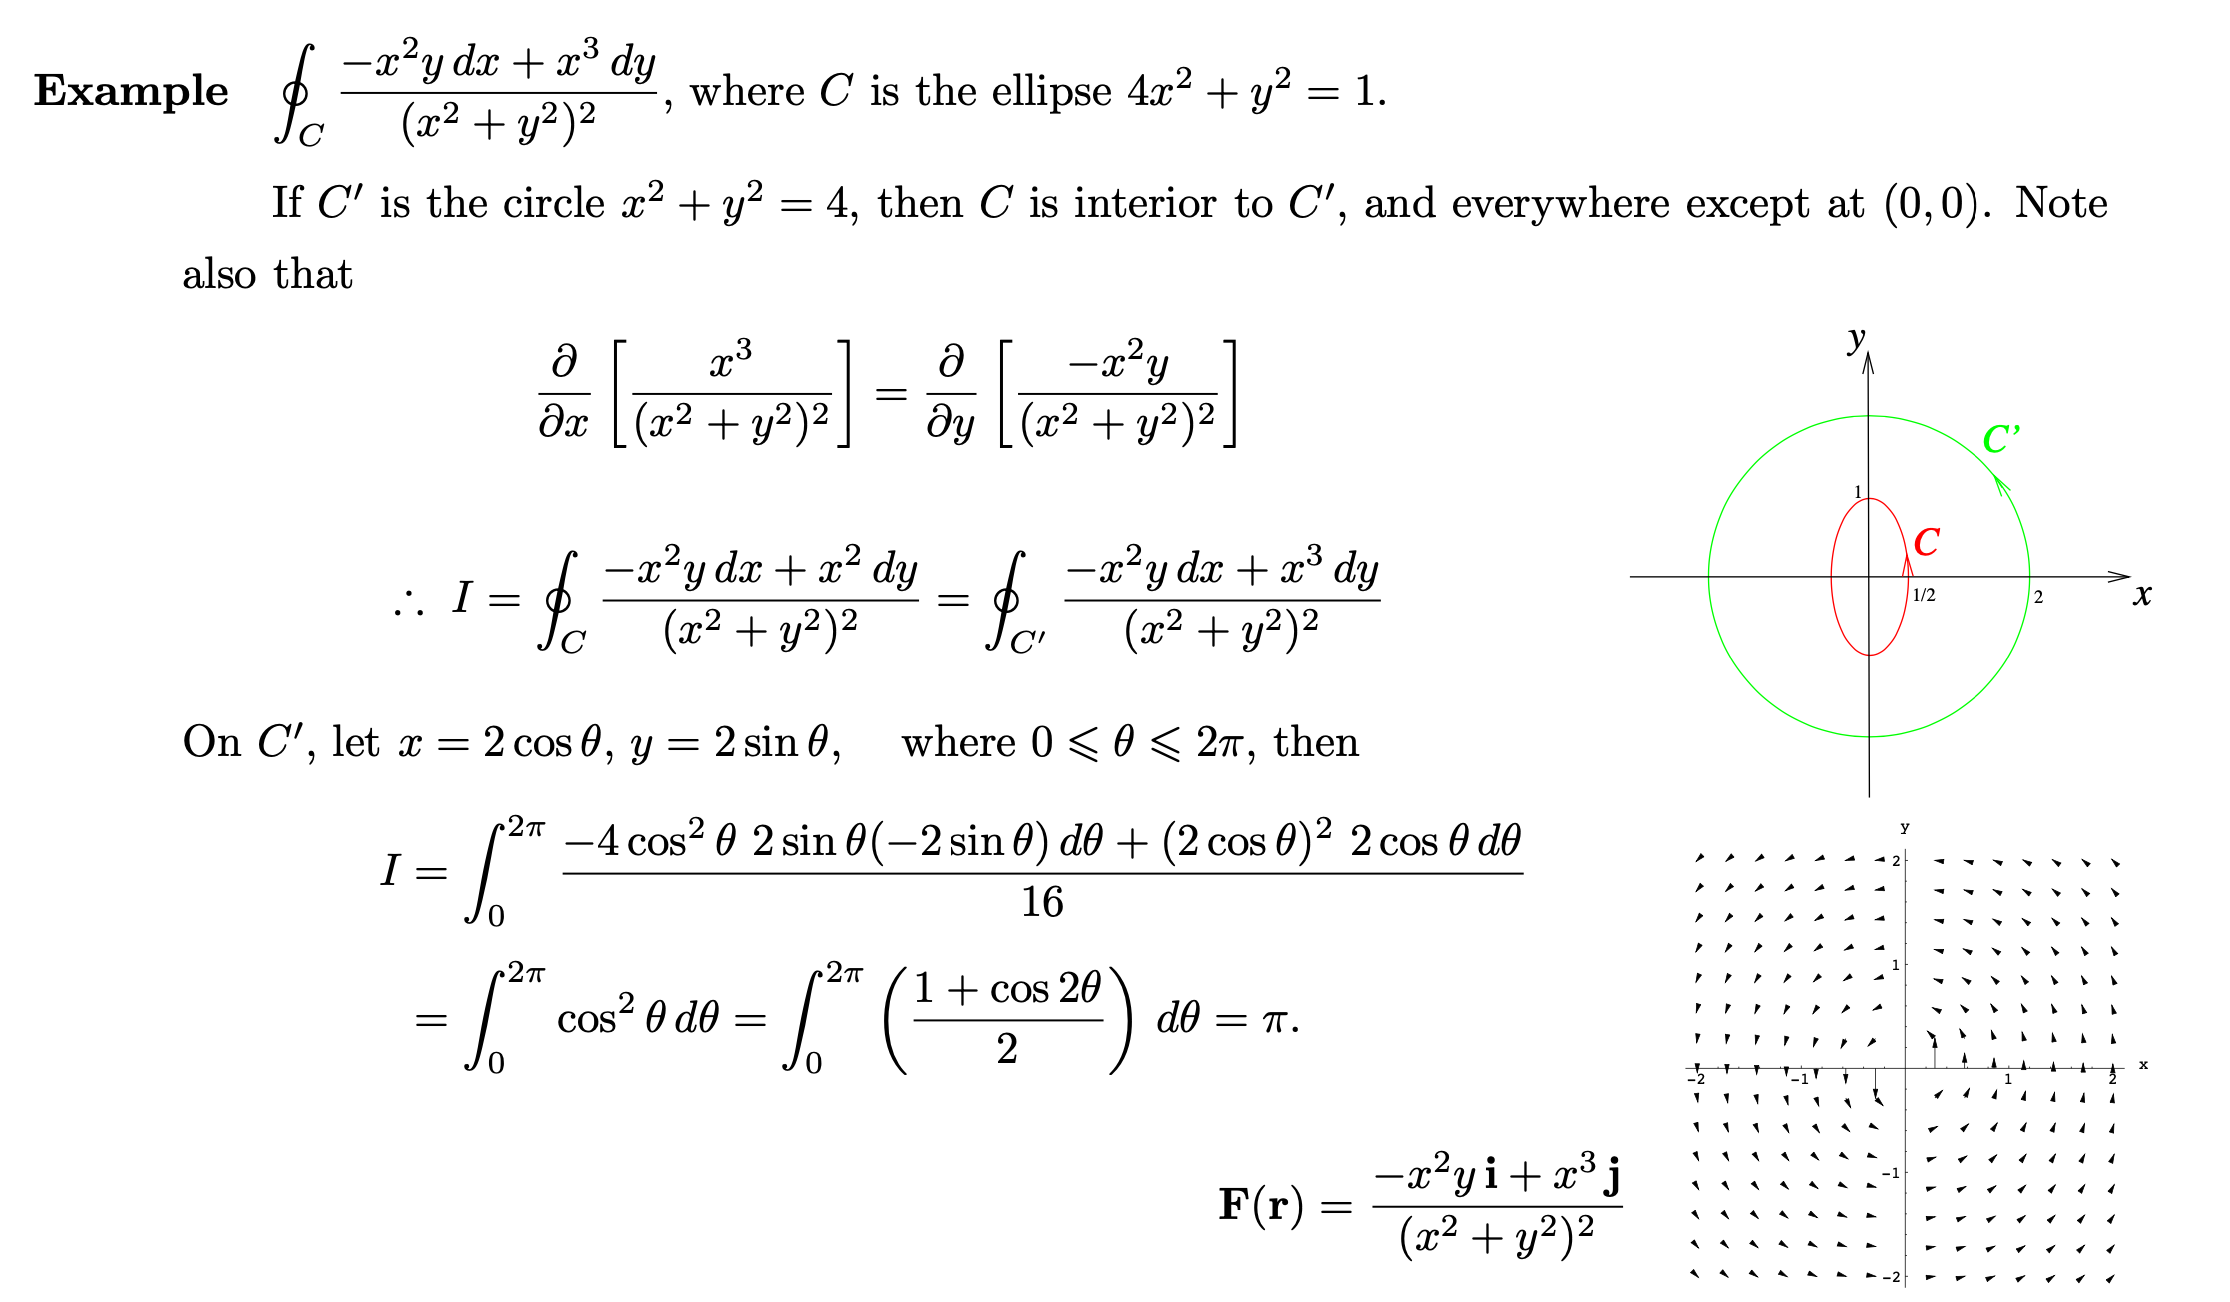
\includegraphics[scale=0.44]{images/Ch16-general-green-eg.png}



    \newpage
    \section{Stokes’ Theorem}
    {\blue Recall in Green's Theorem, 
    $$\oint_C \FF\cdot d\rr =\iint_D (\nabla\times \FF)\cdot \kk dA$$
    where $\FF(\rr)=(F_1,F_2),\ C: \rr(t)=(x(t), y(t)),\ a\le t\le b$}

    Now we want to extends this theorem into 3D space.

    The {\bf Stokes' Theorem} tells that if $S$ is a {\it non-closed} surface, 
    whose boundary consists of a closed smooth curve $C$ with {\it positive orientation,} then
    $$\oint_C \FF\cdot d\rr =\iint_S (\nabla\times \FF)\cdot \nm \ dS$$
    where $\FF(\rr)=(F_1,F_2, F_3),\ C: \rr(t)=\bigl(x(t), y(t), z(t)\bigr),\ a\le t\le b$,
    and $\rr(a)=\rr(b)$ since the boundary is closed. $\nm$ is unit normal vector of surface $S$.

    \vspace{0.4in}
    However, you may have noticed that the theorem doesn't tell how to find $S$. When we evaluate a 
    line integral on $C$, there are lots of surfaces $S$ that can have boundary $C$. 
    \begin{center}
        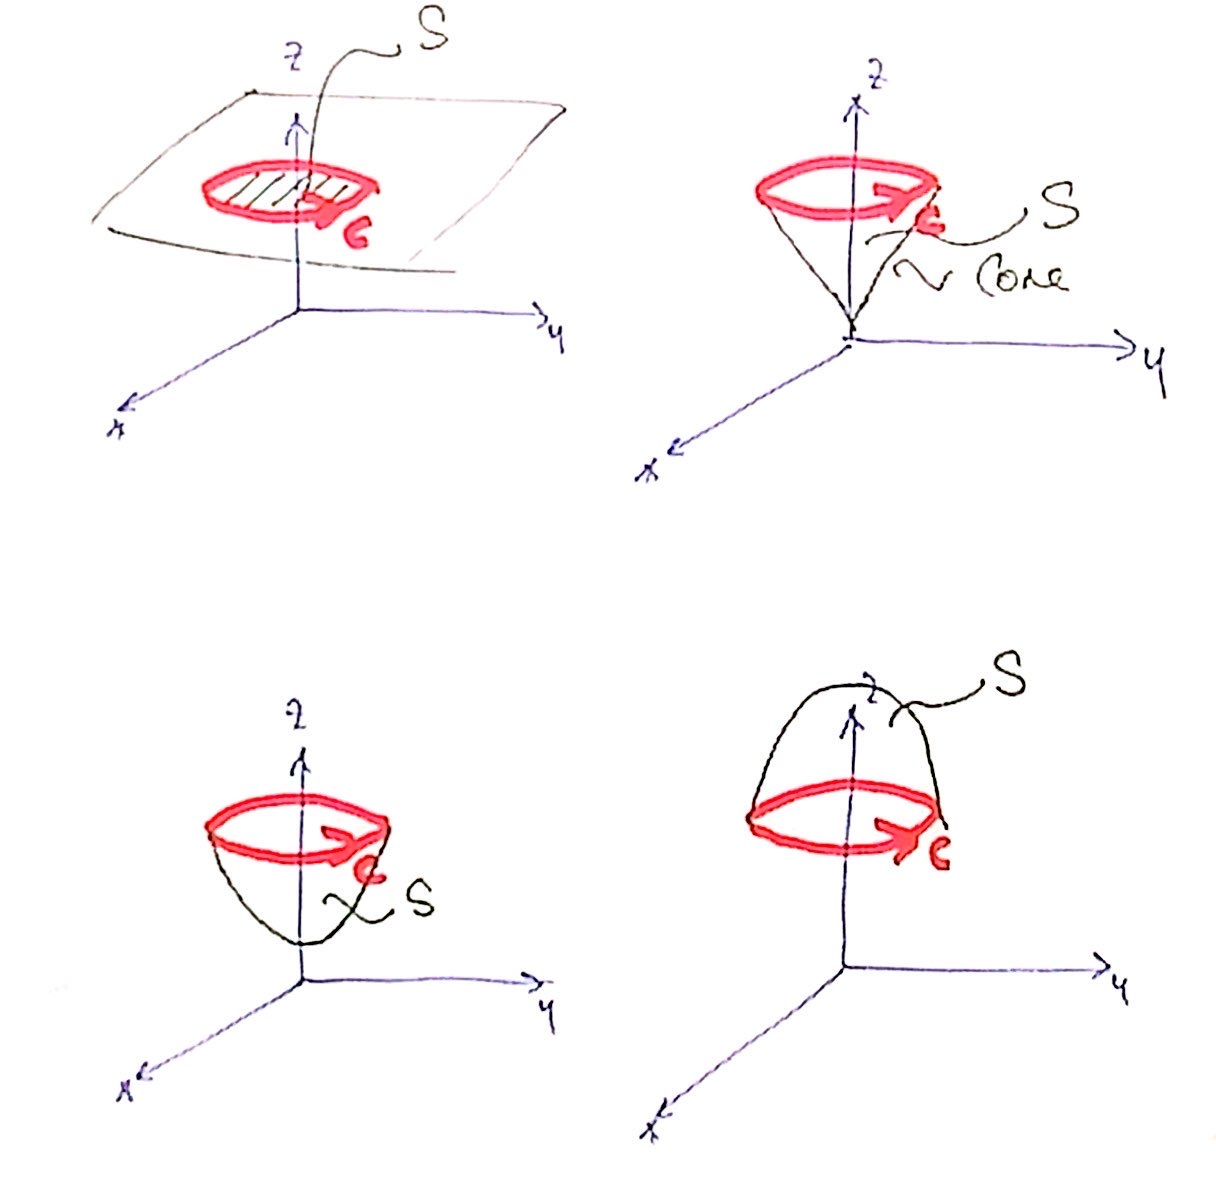
\includegraphics[scale=0.24]{images/Ch16-stoke-manysurfaces.JPG}
    \end{center}

    \newpage
    {\blue This example gives a standard process for applying Stokes' Theorem and provides ideas of 
    how to construct $S$.}

    \eg Find $\disp \oint_C \FF\cdot d\rr$, where $\FF(\rr)=(y,x^2,y)$, $C:\ \rr(t)=(\cos t, \sin t, 1),
    \ 0\le t\le 2\pi$

    \sol {\bf Method 1: } directly compute line integral.
    \begin{align*}
        \oint_C \FF\cdot d\rr &= \int_0^{2\pi} (\sin t, \cos^2 t, \sin t)\cdot (-\sin t, \cos t,0)\ dt\\
        &= \int_0^{2\pi} (-\sin^2 t+\cos^3 t)\ dt
    \end{align*}
    This is tedious.
    
    \vspace{0.3in}
    {\bf Method 2:}
    Notice $\rr(0)=\rr(2\pi)$, so this is a {\it closed curve} in 3D, we can use {\bf Stokes' Theorem}.
    $$\oint_C \FF\cdot d\rr =\iint_S (\nabla\times \FF)\cdot \nm \ dS$$
    {\blue But $S$ is not given, we need to find $S: z=f(x,y)$}

    {\blue Idea: construct 2 surfaces whose {\it intersection} is the curve $C$}.

    From $C$: $\disp \left\{\begin{array}{l}
        x(t)=\cos t\\ y(t)=\sin t\\ z(t)=1
    \end{array} \right.$
    , we can construct 2 surfaces by observing the relationship among $x,y,z$, for example,
    $$\left\{\begin{array}{l}
        x^2+y^2=1\\ z=1
    \end{array} \right. \qquad or \qquad 
    \left\{\begin{array}{l}
        x^2+y^2=1\\ z=x^2+y^2
    \end{array} \right.$$
    Their graphs are shown below:
    \begin{center}
        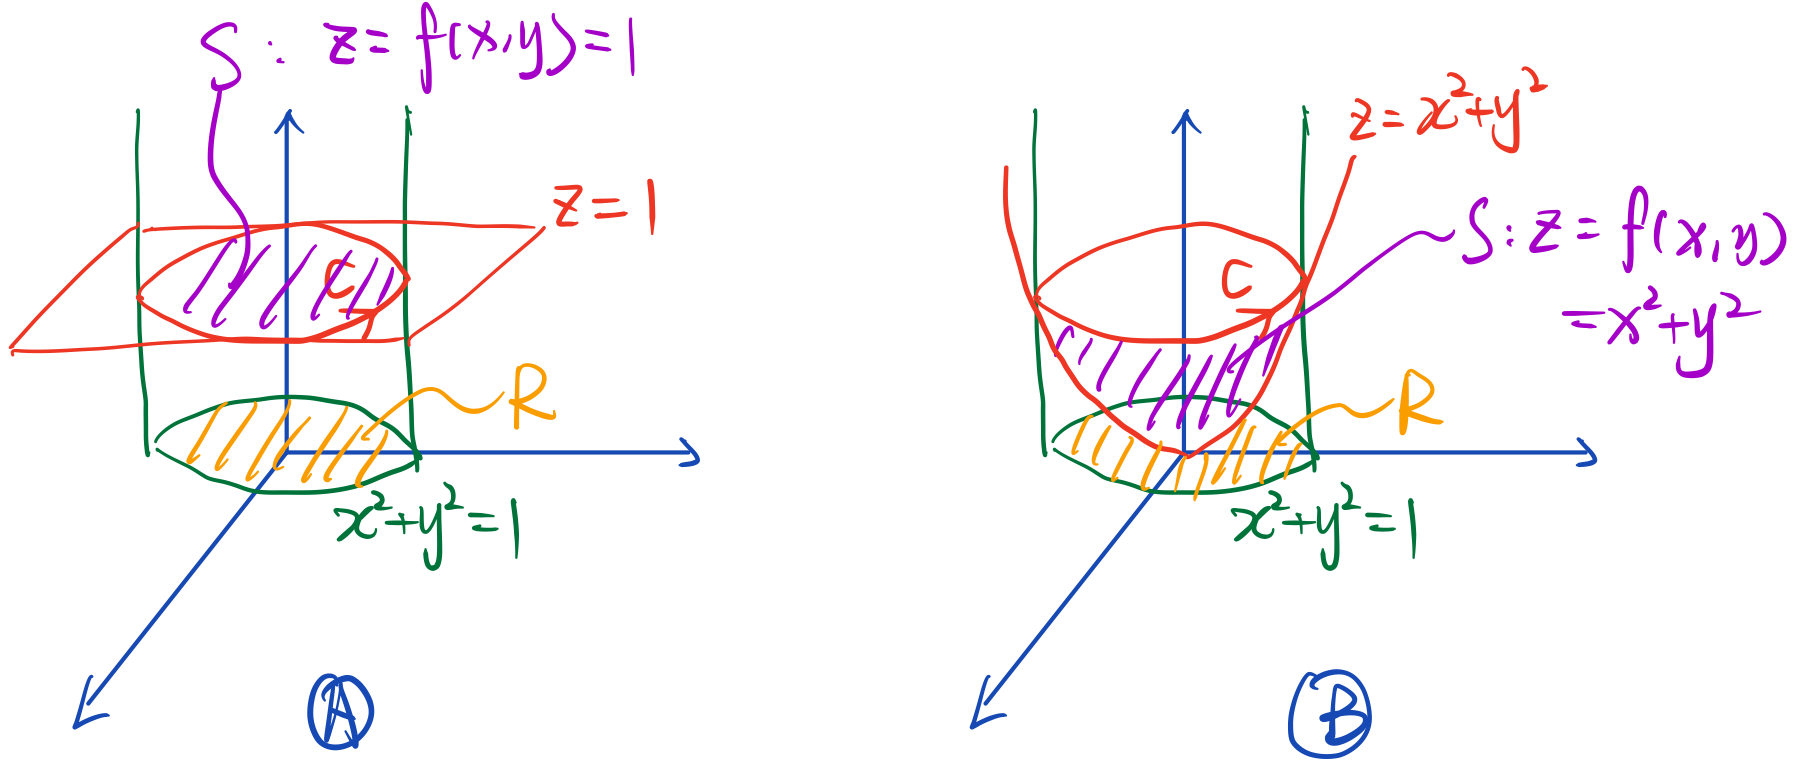
\includegraphics[scale=0.24]{images/Ch16-Stoke-eg.jpeg}
    \end{center}
    We can see that for the first equation, the surface $S$ is a circle, while for the second equation,
    the surface $S$ is a ``rice bowl''. Either of them is ok for our calculation.

    (1) Firstly, find the curl of vector field:
    $$\nabla\times \FF=\left|\begin{array}{ccc}
        \ii & \jj & \kk \\
        \dfrac{\pt }{\pt x} & \dfrac{\pt}{\pt y} & \dfrac{\pt}{\pt z}\\
        y & x^2 & y
    \end{array} \right|=\ii+(2x-1)\kk$$

    (2) Next, find normal vector to the surface,

    \quad For (A), $z=f(x,y)=1$, hence $\nm = \kk$.

    \quad For (B), let $G(x,y,z)=z-x^2-y^2=0$(constant), this is a level set in 3D, hence 
    $${\bf n} =\nabla G=(-2x, -2y, 1),\ \nm =\frac{(-2x,-2y,1)}{\sqrt{1+4x^2+4y^2}}$$

    (3) Then, find surface integral, and thereby calculating the result:

    \quad For (A), $\disp ds=\sqrt{1+(f_x)^2+(f_y)^2} dA=dA$, therefore,
    \begin{align*}
        \iint_S(\nabla \times F)\cdot \nm \ dS &= \iint_R (1,0,2x-1)\cdot (0,0,1)\ dA\\
        &=\iint_R (2x-1)\  dA\\
        &= -\iint_R \ dA = -\pi \qquad {\blue (2x\ \textbf{is\ odd\ in\ {\it x},
        \ and\ the\ region\ is\ symmetric\ w.r.t\ {\it y}})}
    \end{align*}

    \quad For (B), $\disp ds=\sqrt{1+(f_x)^2+(f_y)^2} dA=\sqrt{1+4x^2+4y^2}dA$, therefore,
    \begin{align*}
        \iint_S(\nabla \times F)\cdot \nm \ dS 
        &= \iint_R (1,0,2x-1)\cdot \frac{(-2x,-2y,1)}{\sqrt{1+4x^2+4y^2}}\cdot \sqrt{1+4x^2+4y^2}dA\\
        &=\iint_R (-2x+2x-1)\  dA\\
        &= -\iint_R \ dA = -\pi
    \end{align*}


    \newpage
    \eg Evaluate $\disp \int_{C}(y+\sin x) d x+\left(z^{2}+\cos y\right) d y+x^{3} d z$, 
    where $C:\ \mathbf{r}(t)=(\sin t, \cos t, \sin 2 t), \quad 0 \leqslant t \leqslant 2 \pi$
    
    \sol Note that $C$ is a {\bf closed space curve}, we can view it as circular integration on vector field:
    $$\oint_C (y+\sin x)dx+(z^2+\cos y)dy+x^3 dz=\oint_C \FF\cdot d\rr$$
    where $\FF(x,y,z)=(y+\sin x, z^2+\cos y, x^3)$

    {\bf Step 1:} Find curl of vector field: $\nabla \times \mathbf{F}=\left(-2 z,-3 x^{2},-1\right)$
    
    {\bf Step 2:} To apply Stokes' Theorem, we need to find a surface $S$,

    From $C$: $\disp \left\{\begin{array}{l}
        x(t)=\sin t\\ y(t)=\cos t\\ z(t)=\sin 2t=2\sin t\cos t
    \end{array} \right. \Rightarrow  
    \left\{\begin{array}{l}
        x^2+y^2=1\\ z=1
    \end{array} \right.$
    
    So $C$ can be viewed as the intersection of two surfaces $x^2+y^2=1$ and $z=2xy=f(x,y)$,
    and $z=2xy$ is the $S$ we need, while $R:\ x^2+y^2=1$ is the the projection of $S$
    onto $xy$-plane, which we will need in surface integral.
    \begin{center}
        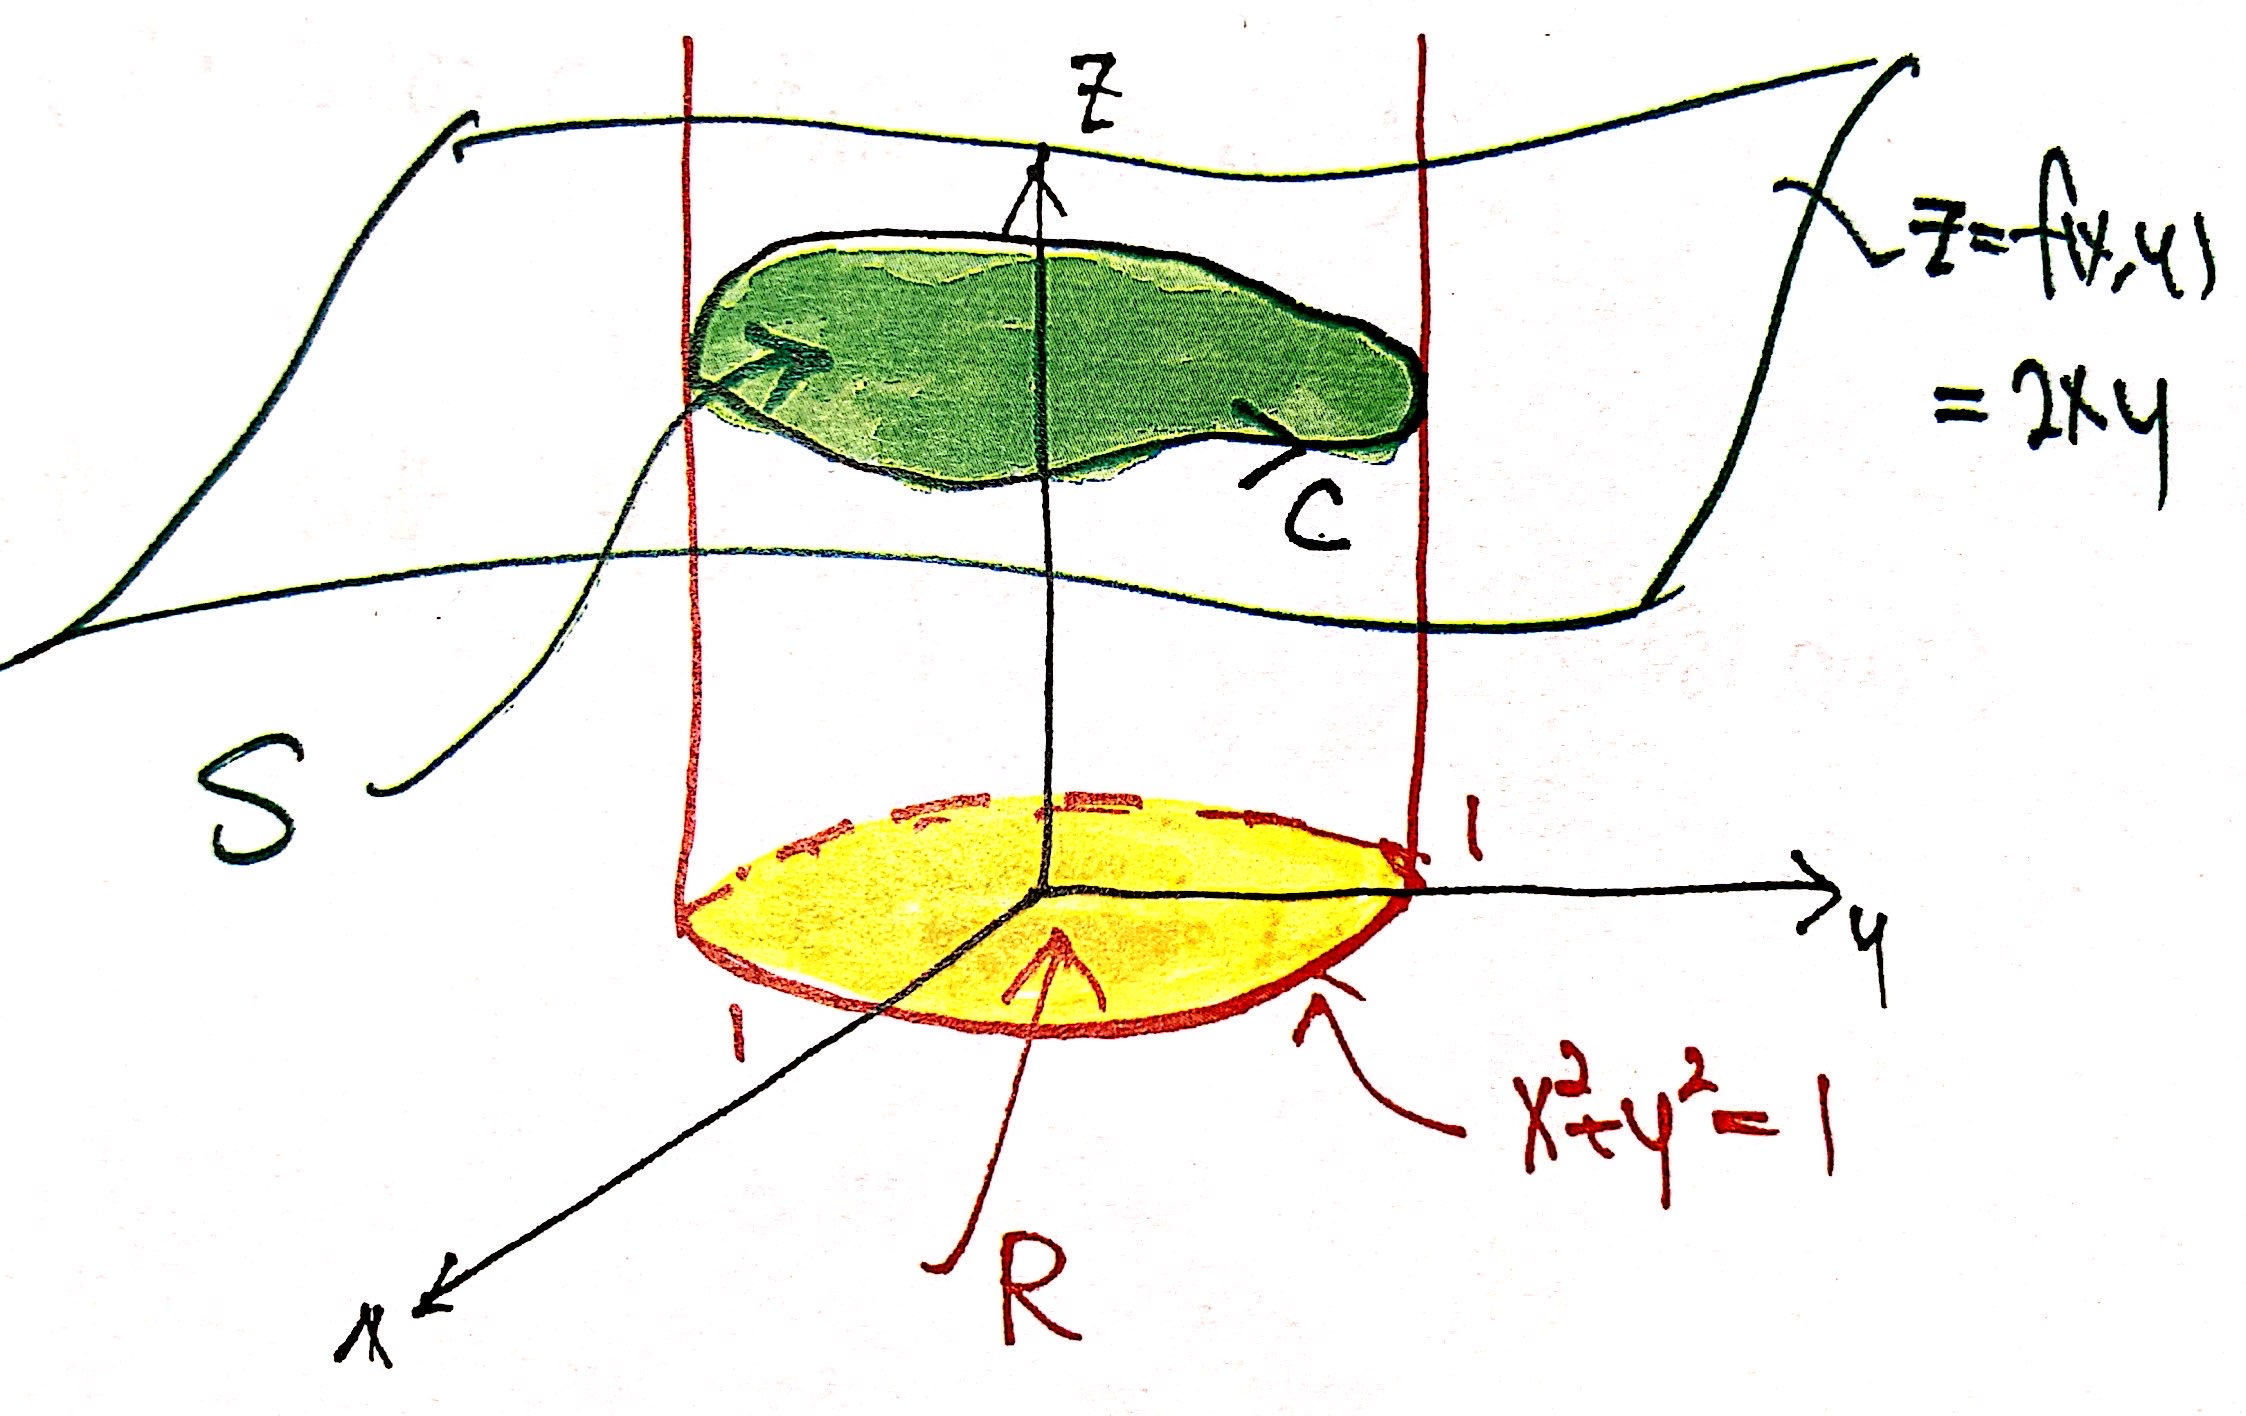
\includegraphics[scale=0.1]{images/Ch16-ex4.5.JPG}
    \end{center}

    {\bf Step 3:} find the normal to $S$:
    
    $f(x, y, z)=z-2 x y=0$(constant) is a level set in 3D, so 
    $$\mathbf{n}=\nabla f=(-2 y,-2 x, 1),\qquad \nm=\frac{(-2 y,-2 x, 1)}{\sqrt{1+4y^2+4x^2}}$$
    
    {\bf Step 4:} find surface integral:
    $dS=\sqrt{1+(f_x)^2+(f_y)^2}\ dA=\sqrt{1+4y^2+4x^2}\ dA$
    Therefore,
    $$\begin{aligned}
    \oint_{C} \mathbf{F} \cdot d \mathbf{r} &=\iint_{S} \nabla \times \mathbf{F} \cdot \widehat{\mathbf{n}} d S \\
    &=\iint_{R}\left(-4 x y,-3 x^{2},-1\right) \cdot \frac{(-2 y,-2 x, 1)}{\sqrt{1+4y^2+4x^2}} \cdot \sqrt{1+4y^2+4x^2}\ dA \\
    &=\iint_{R}\left(8 x y^{2}+6 x^{3}-1\right) d A \\
    &=-\iint_R dA = -\pi\qquad {\blue (same\ trick\ again)}
    \end{aligned}$$

    \newpage
    \vspace*{\fill}
    \begin{center}
        {\it \large This is the end of Chapter 16, and the end of this course!}
    \end{center}

    

\end{spacing}
\end{document}
